% This section is intended to be inserted after the Damsleth gamma-shape
% calibration example in DataAugmentation/Revision/DataAugmentation.tex.
% The figure paths below assume the manuscript is compiled from
% DataAugmentation/Revision.

\subsubsection{Simulation Study}
\label{subsec:gamma-shape-simulation}

We now evaluate the posterior computation problem more systematically.  The
Damsleth examples above are useful calibration cases, but they use fixed
sufficient statistics and therefore do not constitute a repeated simulation
study.  In the experiments below, each one-dimensional posterior distribution
is compared with a grid-based numerical reference for $\xi_2$.  Accuracy is
measured by the Kolmogorov--Smirnov (KS) distance and the Wasserstein-1 (W1)
distance to this numerical reference.  Computational efficiency is measured by
effective sample size per iteration, effective sample size per second, lagged
autocorrelation, and running time.

The main simulation uses
\[
        x_i \stackrel{\rm iid}{\sim} \Gamma(\alpha_{\rm true},1),
        \qquad
        \alpha_{\rm true}\in\{0.1,0.5,1,2,5,20\},
        \qquad
        n\in\{10,50,500\},
\]
with 200 independent data sets in each of the 18 cells.  The methods compared
are the P-IG Gibbs sampler with truncation level $N=200$, slice sampling on
$\log\alpha$, the derivative-matching Gamma approximation of
\cite*{miller2019fast}, the same Miller approximation used as an
independence-Metropolis proposal (Miller-IMH), and the Stirling Gamma
approximation of \cite*{rossell2009gaga}.  All simulations use fixed random
seeds: the full benchmark uses seed 20260430 and initializes task $j$ with
seed $20260430+1009j$.

\begin{table}[t]
        \centering
        \small
        \caption{Main gamma-shape simulation over 18 cells.  KS and W1 are
        measured against the grid reference distribution.  ESS/sec and running
        time are reported only for sampling methods.}
        \label{tab:gamma-shape-main}
        \begin{tabular}{@{}lrrrrr@{}}
                \toprule
                Method & Mean KS & Median KS & Median W1 & Coverage & Median ESS/sec \\
                \midrule
                P-IG Gibbs       & 0.0433 & 0.0250 & 0.0159 & 0.900 & 81.8 \\
                Slice-log-$\alpha$ & 0.0143 & 0.0144 & 0.0062 & 0.906 & 20431.5 \\
                Miller-IMH       & 0.0137 & 0.0137 & 0.0057 & 0.907 & 46916.9 \\
                Miller-Gamma     & 0.0024 & 0.0014 & 0.0019 & 0.909 & -- \\
                Stirling-Gamma   & 0.3358 & 0.1946 & 0.1347 & 0.738 & -- \\
                \bottomrule
        \end{tabular}
\end{table}

Table \ref{tab:gamma-shape-main} shows two distinct facts.  First, the P-IG
Gibbs sampler targets the correct posterior, but at the fixed chain length used
in the main experiment its finite-chain Monte Carlo error is larger than that
of the two generic exact baselines.  The reason is not a change in target
distribution, but slower mixing: the mean lag-1 autocorrelation of P-IG Gibbs
over the main cells is 0.677, compared with 0.004 for slice sampling and 0.011
for Miller-IMH.  Second, in this one-dimensional problem the Miller
approximation is an exceptionally strong problem-specific approximation.  Used
directly as a deterministic approximation, Miller-Gamma has mean KS 0.0024;
used as an independence-Metropolis proposal, Miller-IMH gives an exact sampler
with median ESS/sec 46916.9.  Therefore the main comparison should not be read
as showing that P-IG is the fastest possible one-dimensional sampler.  Rather,
P-IG provides an exact augmentation mechanism for Gamma-function normalizing
constants, whereas Miller-Gamma and Stirling-Gamma are deterministic
approximations to the marginal density.

The distinction between exact augmentation and deterministic approximation is
most visible in the low-shape regime.  We ran an additional stress test with
$\alpha_{\rm true}=0.05$ and $0.10$ and $n=100$.  P-IG Gibbs, slice sampling,
and Miller-IMH all remained close to the grid reference, with mean KS around
0.013--0.014 and empirical 95\% coverage equal to 1.00.  Miller-Gamma was also
accurate in these one-dimensional cases, with mean KS 0.0006.  In contrast,
Stirling-Gamma failed badly: its KS distance was 0.978 at
$\alpha_{\rm true}=0.05$ and 0.951 at $\alpha_{\rm true}=0.10$, with zero
coverage in both cells.  Thus the simulations identify the main failure mode
of the older approximation: Stirling's formula is not reliable when the shape
parameter is small.

To separate exactness from finite-chain efficiency, we fixed three
representative posterior targets and ran P-IG Gibbs for 5000, 20000, and
100000 iterations with four independent chain seeds.  Miller-Gamma and
Stirling-Gamma were evaluated once on the same fixed targets.  The results are
reported in Table \ref{tab:gamma-shape-exactness} and Figure
\ref{fig:gamma-shape-exactness}.  The P-IG error decreases as the chain length
increases.  For the low-shape target, P-IG KS drops from 0.0139 at 5000
iterations to 0.0034 at 100000 iterations, while the Stirling approximation
remains at KS 0.954.  For the high-shape large-$n$ target, P-IG KS drops from
0.1401 to 0.0164, whereas Stirling-Gamma remains at 0.0545.  This is the key
benefit of exact augmentation: P-IG error is Monte Carlo error around the exact
posterior and can be reduced with more simulation; approximation error is an
algorithmic bias and does not vanish by running a chain longer.

\begin{table}[t]
        \centering
        \small
        \caption{Fixed-target chain-length experiment.  P-IG Gibbs is run with
        four independent chains at each iteration count.  Miller-Gamma and
        Stirling-Gamma are deterministic approximations evaluated on the same
        targets.}
        \label{tab:gamma-shape-exactness}
        \begin{tabular}{@{}llrrrrr@{}}
                \toprule
                Target & Method & Iter. & KS & W1 & Coverage & Median runtime \\
                \midrule
                Low shape & P-IG Gibbs & 5000   & 0.0139 & 0.00022 & 1.00 & 6.25 \\
                Low shape & P-IG Gibbs & 20000  & 0.0073 & 0.00011 & 1.00 & 20.93 \\
                Low shape & P-IG Gibbs & 100000 & 0.0034 & 0.00004 & 1.00 & 92.22 \\
                Low shape & Miller-Gamma   & -- & 0.0009 & 0.00003 & 1.00 & -- \\
                Low shape & Stirling-Gamma & -- & 0.9536 & 0.03718 & 0.00 & -- \\
                \midrule
                Moderate shape & P-IG Gibbs & 5000   & 0.0506 & 0.11196 & 1.00 & 4.63 \\
                Moderate shape & P-IG Gibbs & 20000  & 0.0286 & 0.06794 & 1.00 & 16.27 \\
                Moderate shape & P-IG Gibbs & 100000 & 0.0109 & 0.03383 & 1.00 & 66.41 \\
                Moderate shape & Miller-Gamma   & -- & 0.0011 & 0.00467 & 1.00 & -- \\
                Moderate shape & Stirling-Gamma & -- & 0.0500 & 0.15793 & 1.00 & -- \\
                \midrule
                High shape, large $n$ & P-IG Gibbs & 5000   & 0.1401 & 0.36471 & 1.00 & 23.60 \\
                High shape, large $n$ & P-IG Gibbs & 20000  & 0.1062 & 0.29488 & 1.00 & 83.04 \\
                High shape, large $n$ & P-IG Gibbs & 100000 & 0.0164 & 0.04557 & 1.00 & 440.33 \\
                High shape, large $n$ & Miller-Gamma   & -- & 0.0002 & 0.00041 & 1.00 & -- \\
                High shape, large $n$ & Stirling-Gamma & -- & 0.0545 & 0.16389 & 1.00 & -- \\
                \bottomrule
        \end{tabular}
\end{table}

\begin{figure}[t]
        \centering
        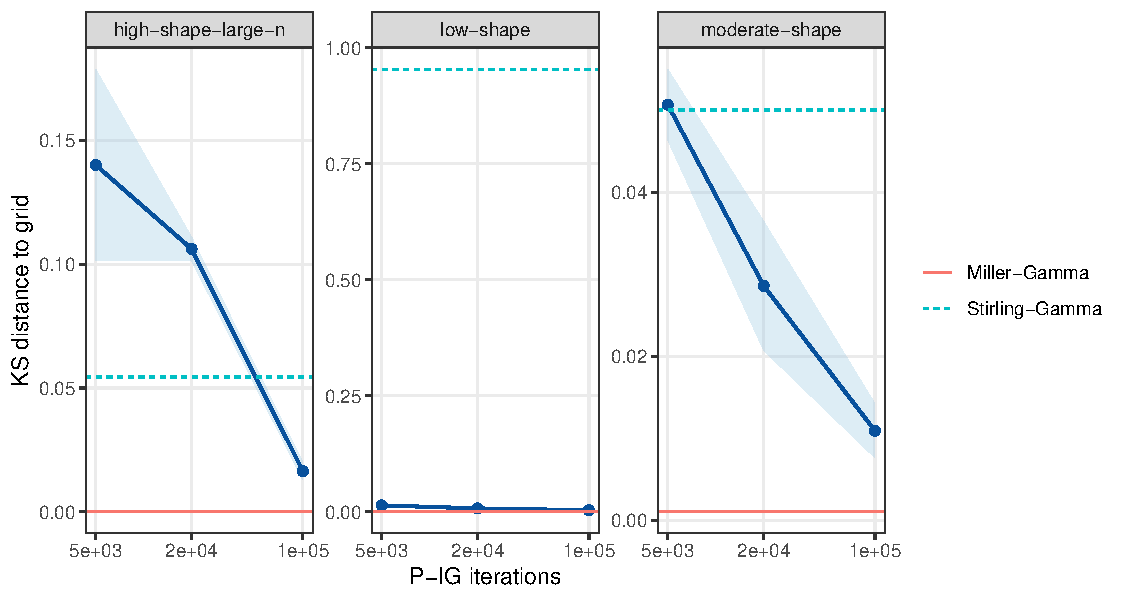
\includegraphics[width=0.88\linewidth]{../../code2026/gamma_shape_inference/results/manuscript_tables/figures/pig_exactness_ks_vs_iterations.pdf}
        \caption{P-IG Monte Carlo error decreases with chain length, while
        deterministic approximation error remains fixed.  The blue curves show
        P-IG KS distance to the grid reference at 5000, 20000, and 100000
        iterations; horizontal lines show Miller-Gamma and Stirling-Gamma on
        the same fixed targets.}
        \label{fig:gamma-shape-exactness}
\end{figure}

We also varied the P-IG truncation level
$N\in\{50,100,200,500,1000\}$.  The mean KS distances were 0.0599, 0.0574,
0.0579, 0.0541, and 0.0585, respectively, while median runtimes increased from
1.13 seconds at $N=50$ to 16.70 seconds at $N=1000$.  At the chain lengths used
here, increasing $N$ beyond 200 does not produce a visible improvement in
posterior accuracy; the remaining error is dominated by Monte Carlo error.
Thus $N=200$ is a reasonable default for the simulations reported above.

Finally, the informative-prior experiment clarifies the current scope of the
Gibbs construction.  The P-IG update above introduces $\delta'$ independent
P-IG variables and is therefore exact for integer posterior sample size
$\delta'$.  In the prior robustness experiment, all non-integer posterior
$\delta'$ cases arising from prior $\delta=0.5$ and $2.5$ were marked as
outside the present exact Gibbs construction.  Integer posterior cases
corresponding to prior $\delta=10$ and $50$ ran normally and remained close to
the grid reference.  We therefore state the integer-$\delta'$ condition
explicitly: extending the augmentation to non-integer posterior sample size is
a separate direction, whereas the present contribution is an exact Gibbs
augmentation for the integer-$\delta'$ Gamma-shape posterior and for the larger
Gamma-function models covered by Proposition \ref{prop:cond}.
